

%%%%%%%%%%%%%%%%%%%%%%%%%%%%%%%%%%%%%%%%%%%%%%%%%%%%%%%%%%%%%%%%%%%%%%
%%%%%%%%%%%%%%%% Supportive information
%%%%%%%%%%%%%%%%%%%%%%%%%%%%%%%%%%%%%%%%%%%%%%%%%%%%%%%%%%%%%%%%%%%%%%
\section{Additional information}
\label{sec:support}


\subsection{An 8-layer Convolutional neural network}

The architecture of the 8-layer convolutional neural network used in the classification of CIFAR dataset is presented in Table \ref{tab:8layer}.

% Please add the following required packages to your document preamble:
%%%%%%%% Table 8-layer CNN
\begin{table}[t]
\resizebox{\columnwidth}{!}{
\centering
\begin{tabular}{c|c|c}
\hline
layer name             & output size                     & 8-layer                               \\ \hline
\multirow{3}{*}{conv1} & \multirow{3}{*}{16 $\times$ 16} & 3 $\times$ 3, 32, LeakyReLU(0.2)      \\ \cline{3-3}
                       &                                 & 3 $\times$ 3, 32, LeakyReLU(0.2)      \\ \cline{3-3}
                       &                                 & 2 $\times$ 2 max pool, dropout(0.2)   \\ \hline
\multirow{3}{*}{conv2} & \multirow{3}{*}{8 $\times$ 8}   & 3 $\times$ 3, 64, LeakyReLU(0.2)      \\ \cline{3-3}
                       &                                 & 3 $\times$ 3, 64, LeakyReLU(0.2)      \\ \cline{3-3}
                       &                                 & 2 $\times$ 2 max pool, dropout(0.2)   \\ \hline
\multirow{3}{*}{conv3} & \multirow{3}{*}{4 $\times$ 4}   & 3 $\times$ 3, 128, LeakyReLU(0.2)     \\ \cline{3-3}
                       &                                 & 3 $\times$ 3, 128, LeakyReLU(0.2)     \\ \cline{3-3}
                       &                                 & 2 $\times$ 2 max pool, dropout(0.2)   \\ \hline
\multirow{2}{*}{fc}    & \multirow{2}{*}{1 $\times$ 1}   & flatten, 512-d fc, ReLU, dropout(0.5) \\ \cline{3-3}
                       &                                 & 11-d fc, softmax                      \\ \hline
\multicolumn{2}{c|}{Parameters}                          & 1,341,739                             \\ \hline
\end{tabular}
}
\caption{8-layer Convolutional Neural Networks used in the CIFAR dataset classification.}
\label{tab:8layer}
\end{table}

\subsection{Evaluation metrics}

% \noindent (overall) accuracy
$$ \text{accuracy} = \frac{\text{true pos. + true neg.}}{\text{true pos. + false pos. + true neg. + false neg.}}$$

% \noindent precision
$$\text{precision} = \frac{\text{true pos.}}{\text{true pos. + false pos.}}$$

% \noindent recall
$$\text{recall} = \frac{\text{true pos.}}{\text{true pos. + false neg.}}$$

% \noindent f1-score
$$F_1 = 2 \cdot \frac{\text{precision} \cdot \text{recall}}{\text{precision}+\text{recall}}$$

% \noindent intersection over union (IU)
$$ \text{IU} = \frac{\text{true pos.}}{\text{true pos. + false pos. + false neg.}}$$



%%%%%%%%%%%%%%%%%%%%%%%%%%%%%%%%%%%%%%%%%%%%%%%%%%%%%%%%%%%%%%%%%%%%%%
%%%%%%%%%%%%%%%% Appendix Results                     %%%%%%%%%%%%%%%%
%%%%%%%%%%%%%%%%%%%%%%%%%%%%%%%%%%%%%%%%%%%%%%%%%%%%%%%%%%%%%%%%%%%%%%

% \section{Additional Results}
% \label{sec:addition}
%
% %%%%%%%% FIGURE Number of training categories
% \begin{figure}[t]
% \centering
%    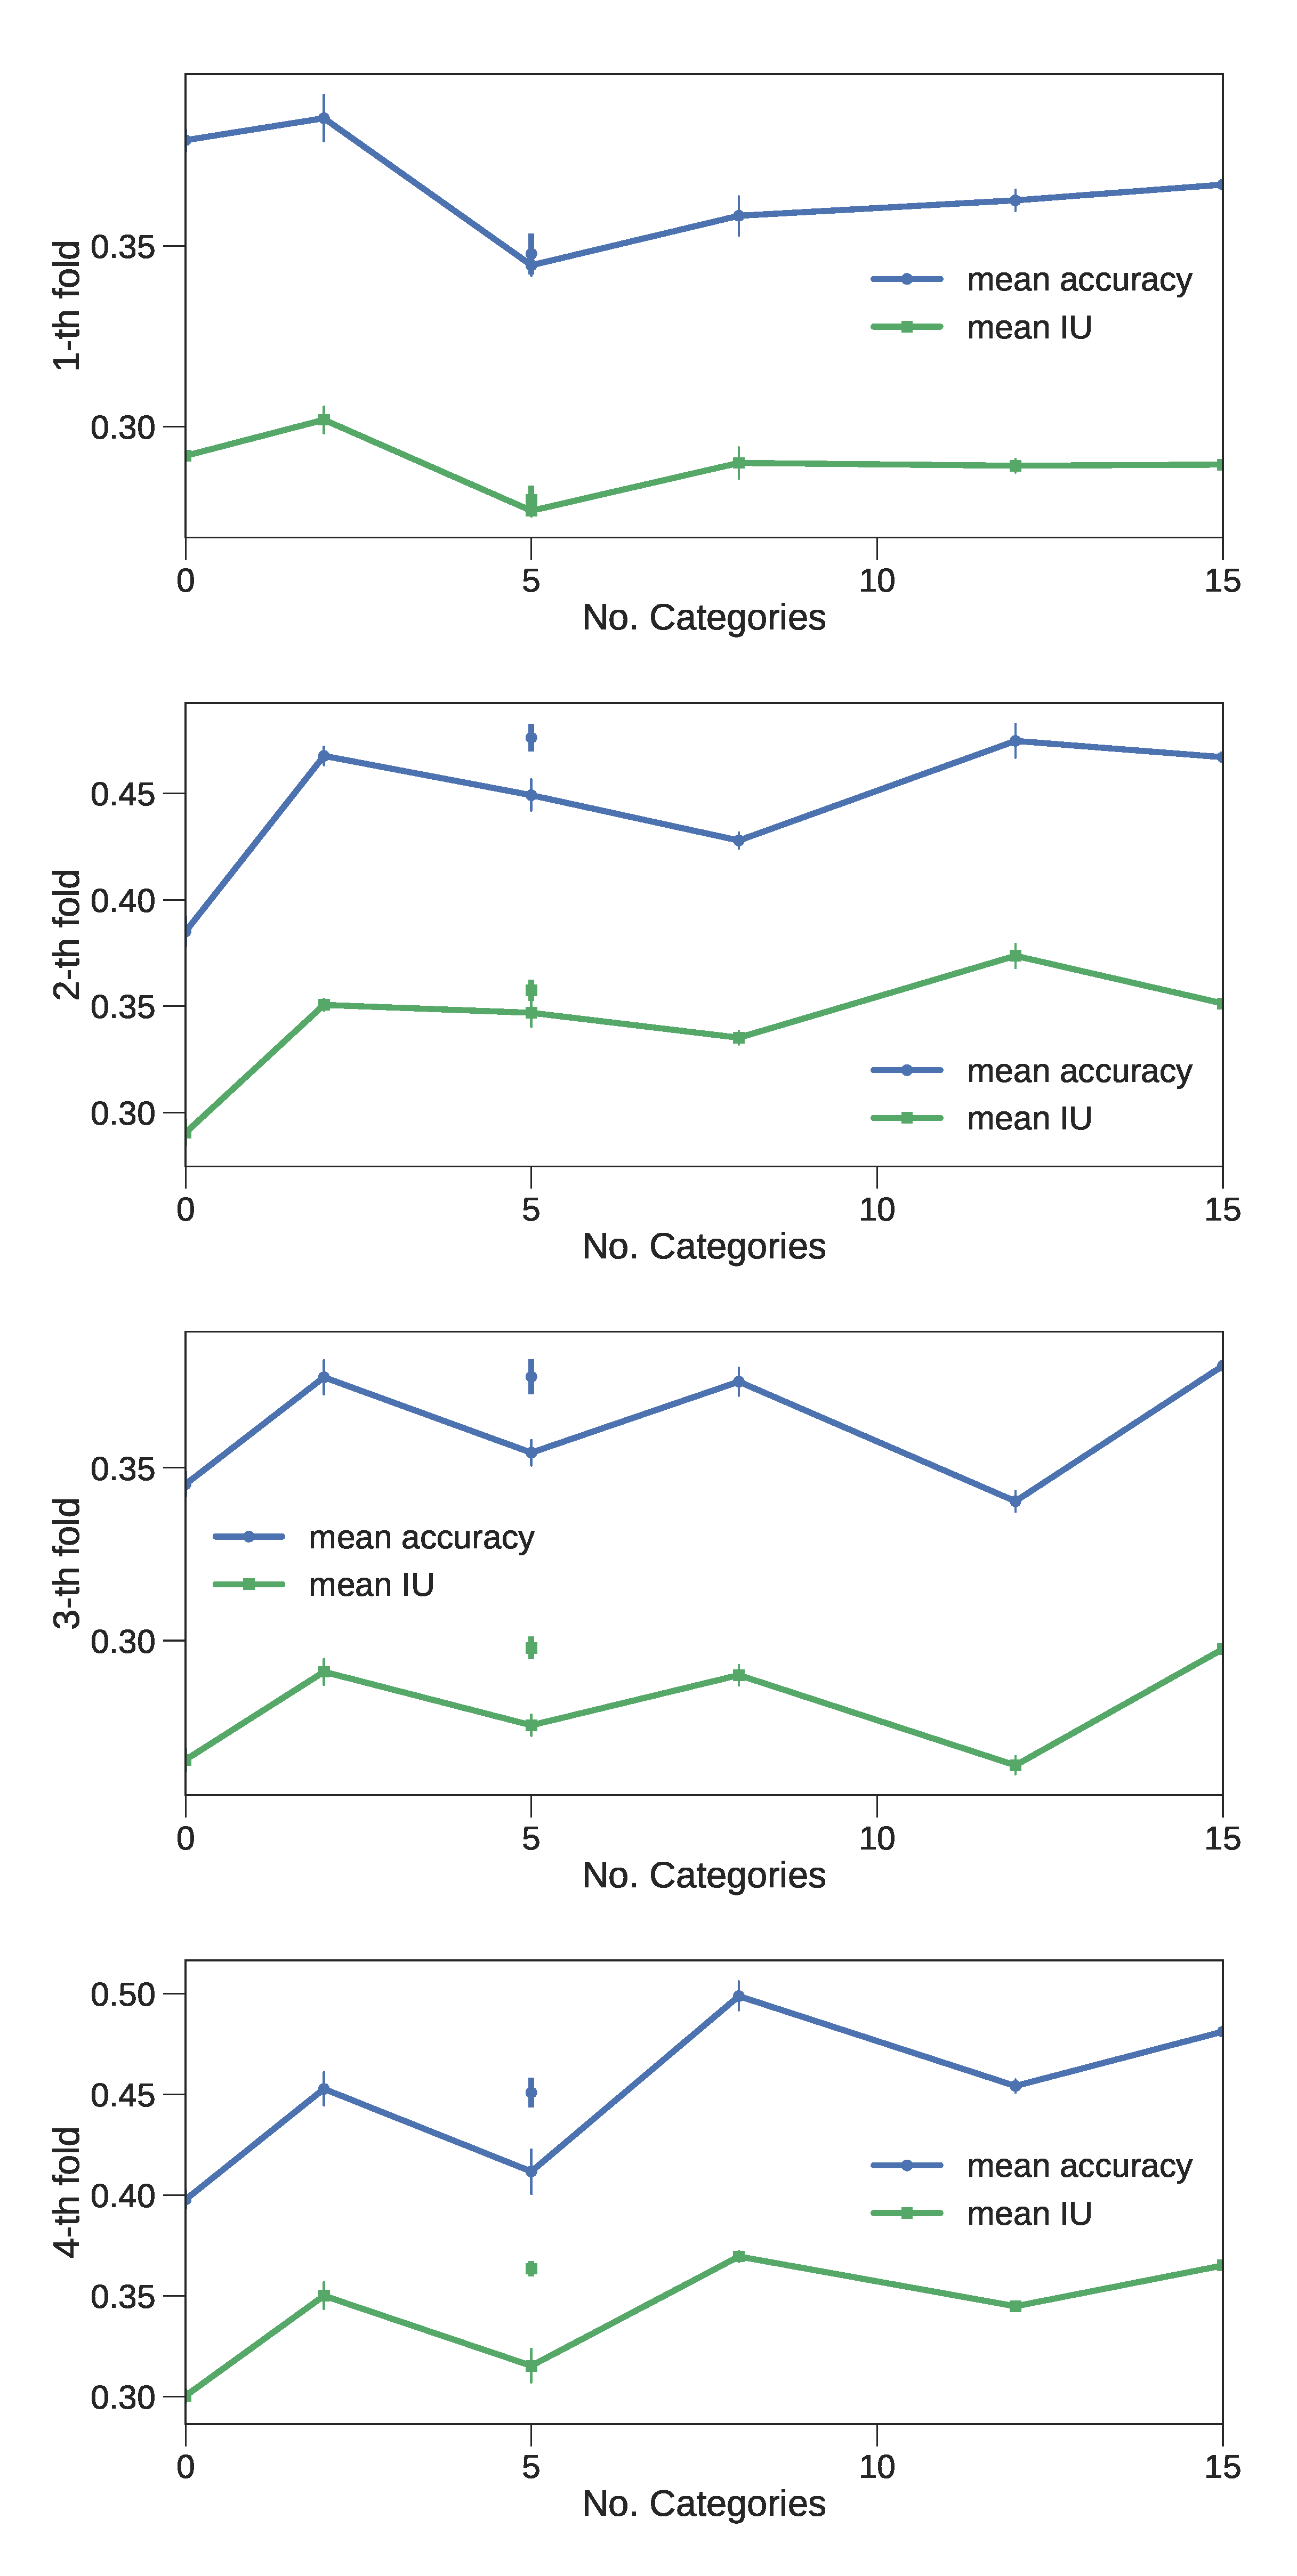
\includegraphics[width=\linewidth]{img/num_classes_folds.eps}
% \caption{The influence of categorizing classes on test performance of fine-tuned models for each fold, addition to Figure \ref{fig:categories}.}
% \label{fig:classesfold}
% \end{figure}
